\documentclass[reprint, aps, prd, nofootinbib, superscriptaddress, floatfix]{revtex4-2}  % chktex 8

\usepackage{graphicx}% Include figure files
\usepackage{dcolumn}% Align table columns on decimal point
\usepackage{bm}% bold math
\usepackage[linktocpage,colorlinks,pdfusetitle,allcolors=blue]{hyperref}
\usepackage{amsmath, amssymb}
\usepackage{siunitx}
\usepackage{cancel}


\renewcommand{\d}[1]{\ensuremath{\operatorname{d}\!{#1}}}
\renewcommand{\vec}[1]{\boldsymbol{#1}}

\newlength\figureheight
\newlength\figurewidth
\setlength\figureheight{\linewidth}
\setlength\figurewidth{\linewidth}


\newcommand{\eq}[1]{Eq.\ \eqref{#1}}
\newcommand{\fig}[1]{Fig.\ \ref{#1}}
\newcommand{\SV}[1]{{\color{red}{[[Stamatis:: #1]]}}}
\newcommand{\BK}[1]{{\color{green}{[[Badri:: #1]]}}}
\newcommand{\GB}[1]{{\color{blue}{[[Erik:: #1]]}}}
\newcommand{\Mdot}{\langle \dot{M} \rangle}
\newcommand{\Jdot}{\langle \dot{J} \rangle}




\begin{document}

\title{Report}

\author{Stamatis Vretinaris}
\email{svretina@physics.auth.gr}
\affiliation{
  Institute for Mathematics, Astrophysics and Particle Physics, Radboud University, Heyendaalseweg 135, 6525 AJ Nijmegen, The Netherlands
}


\date{\today}

\begin{abstract}

\end{abstract}

\maketitle
\section{Introduction}
We solve the simple wave equation
\begin{equation}
  \label{eq:wave-equation}
  u_{tt} - u_{xx} = 0
\end{equation}
where subscripts indicate derivatives $u_x = \partial u /\partial x$. We recast it to a first order system
\begin{align}
  \label{eq:1st-order-system}
  \pi &:= \partial_t u \nonumber \\
  \xi &:= \partial_x u \\
  \pi_t &= \partial_x \xi \nonumber\\
  \xi_t &= \partial_x \pi \nonumber
\end{align}
and evolve it in time with a Runge-Kutta integrator of 4th order.

The initial conditions are given as a Gaussian pulse travelling to the right.
\begin{align}
  \label{eq:initial-conditions}
  u(x,0) &= f(x) = A \exp[-(x-t)^2/\sigma] \\
  u_t(x,0) &= \pi(x,0) = f'(x) = \frac{2 (x-t)}{\sigma} f(x)
\end{align}

We assume throught this report a Courant factor of 0.4, a domain $x\in[0,1]$ and the time step is then given by
\begin{equation}
  \label{eq:timestep}
  dt = \mathcal{C} dx,
\end{equation}
where $\mathcal{C}$ is the Courant factor.


\section{Boundary Conditions}
We use radiative/absorbing boundary conditions. Namely we use
\begin{equation}
  \label{eq:boundary-condition}
  u_{xt} - u_{xx} = 0.
\end{equation}
Using Eq. \ref{eq:1st-order-system} we can rewrite Eq. \ref{eq:boundary-condition}
\begin{align}
  \label{eq:bc-left}
  \pi_t - \xi_t &= 0, \\
  \pi_t + \xi_t &= \xi_x + \pi_x,
\end{align}
for the left boundary $x=0$ and
\begin{align}
  \label{eq:bc-right}
  \pi_t - \xi_t &= \xi_x - \pi_x, \\
  \pi_t + \xi_t &= 0,
\end{align}
for the right boundary $x=L=1$. Combining these formulas we derive the expressions for the boundary
\begin{equation}
  \label{eq:rhs-bc-left}
  \begin{split}
    \pi_t &= \frac{1}{2} (\xi_x + \pi_x), \\
    \xi_t &= \frac{1}{2} (\xi_x + \pi_x),
  \end{split}
\end{equation}
for the left boundary and
\begin{equation}
  \label{eq:rhs-bc-right}
  \begin{split}
    \pi_t &= \frac{1}{2} (\xi_x - \pi_x), \\
    \xi_t &= \frac{1}{2} (\pi_x - \xi_x),
  \end{split}
\end{equation}
for the right boundary. We apply these boundary conditions by modifying the right hand side function in our evolution scheme. This is known as imposing boundary conditions \textit{strongly}.
\section{Convergence}
We will denote the analytical solution as $\tilde{u}$ and the numerical solution which depends on $h=dx$ as $u_h$. If the numerical method is of order $p$, then there exists a number $C$ such that
\begin{equation}
  \label{eq:conv-cond}
  |u_h - \tilde{u}| \leq C h^p.
\end{equation}
Assuming that the error $|u_h - \tilde{u}|$ depends smoothly on $h$
\begin{equation}
  \label{eq:conv-cond2}
  u_h - \tilde{u} = C h^p + \mathcal{O}(h^{p+1}).
\end{equation}
If the exact solution $\tilde{u}$ is known, then check the sequence
\begin{equation}
  \label{eq:conv-log}
  \log|u_h-\tilde{u}| = \log|C|+p\log h + \mathcal{O}(h),
\end{equation}
for different values of $h$ and fit a linear functions of $\log h$ to approximate $p$.
In order to study the convergence of our code we fit a linear function to the sequence of Eq. \ref{eq:conv-log} for $h=[h/2, h/4, h/6, h/8, h/10]$ at an instance of time. For example, for t=1 we get the following convergence as seen in Fig. \ref{fig:l2-convergence-t=1}
\begin{figure*}[htbp]
  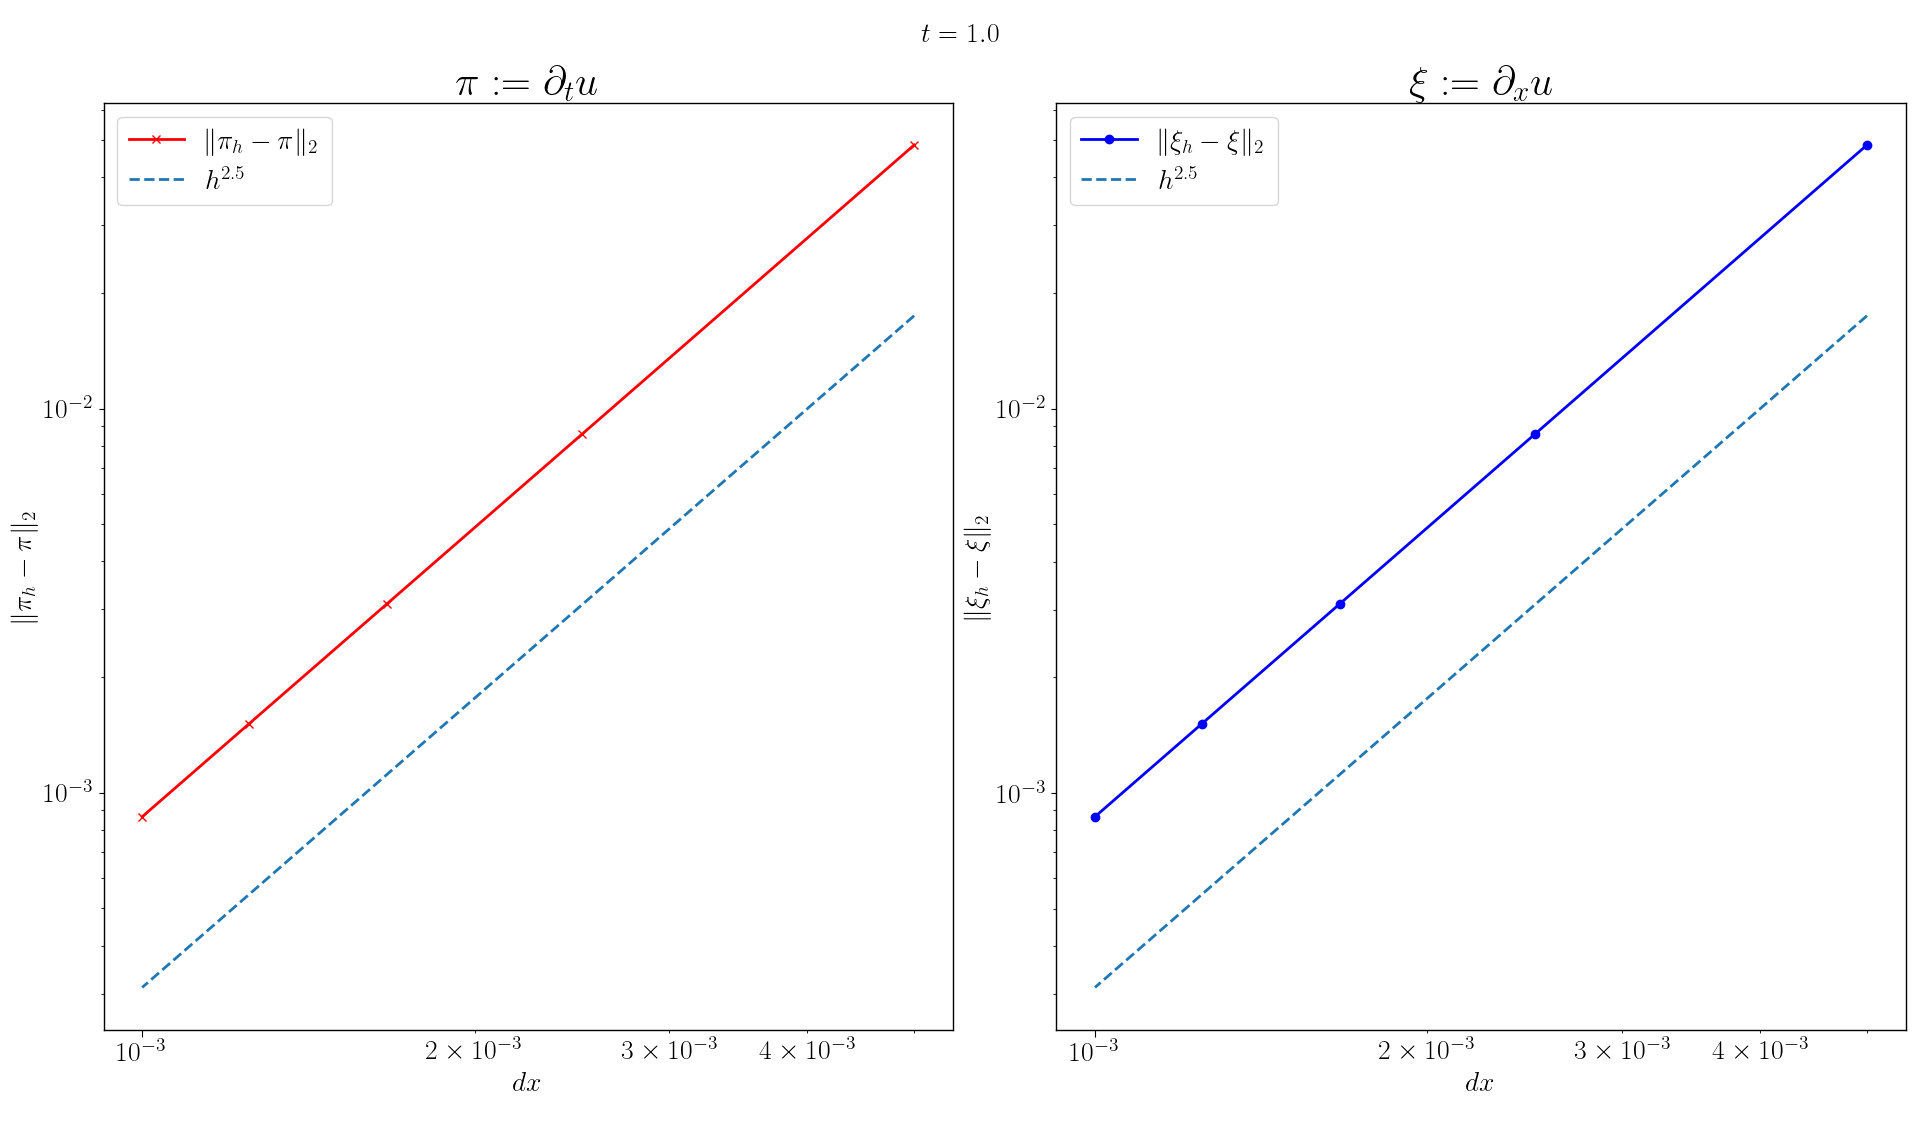
\includegraphics[width=16cm]{./L2_convergence.png}
  \caption{Convergence of $L_2$ norm for t=1. The left subfigure shows the convergence of $\pi$ and the right subfigure shows the convergence of $\xi$. We see here that the convergence is p=2.5.}
  \label{fig:l2-convergence-t=1}
\end{figure*}
We repeat this calculation of the convergece $p$, for all time instances and get a non constant convergence over time as seen in Fig. \ref{fig:l2-convergence-t}.
\begin{figure*}[htbp]
  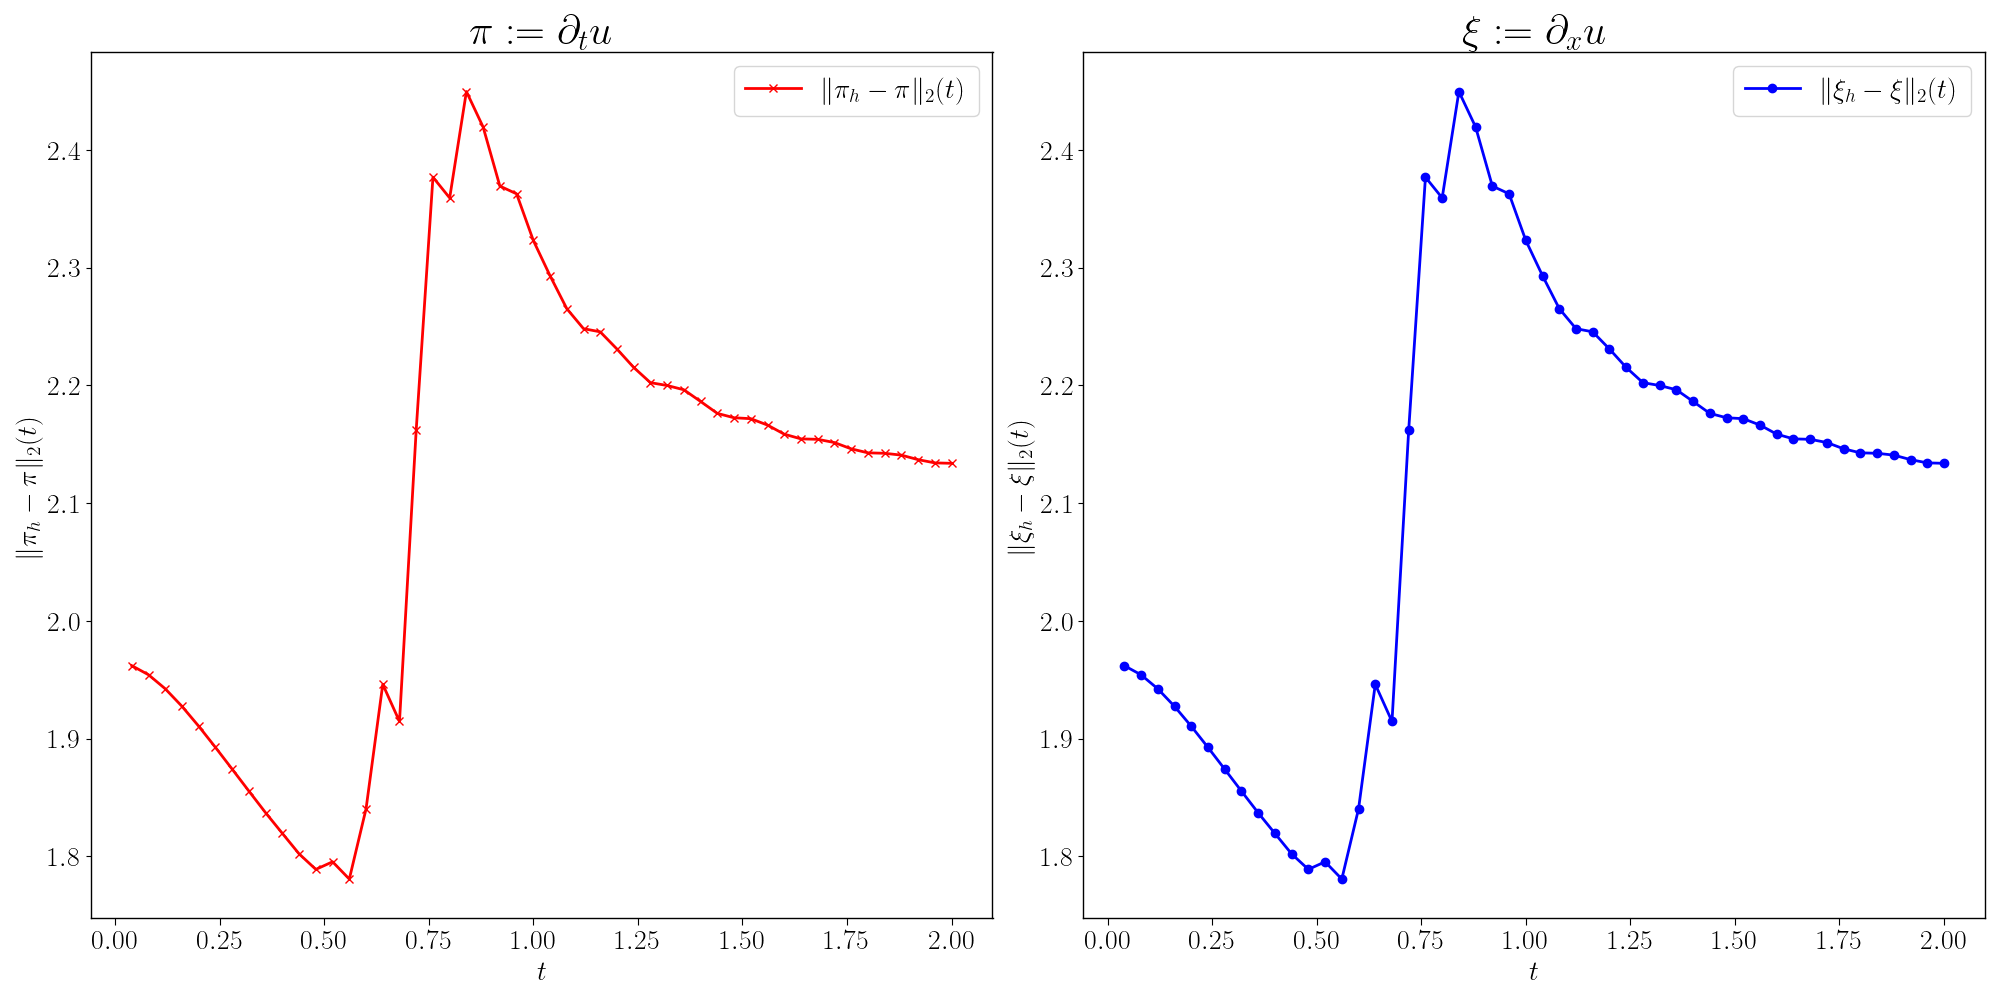
\includegraphics[width=16cm]{./L2_convergence_over_time.png}
  \caption{Convergence of $L_2$ norm for t=1. The left subfigure shows the convergence over time of $\pi$ and the right subfigure shows the convergence over time of $\xi$. We see that it is not constant.}
  \label{fig:l2-convergence-t}
\end{figure*}

\end{document}